% Ajit and Craig's section

\graphicspath{{11-Absorber/Figures/}}

\section{Liquid Hydrogen absorber}
\label{Sect:Absorber}

\subsection{Introduction}
As a muon beam passes through material, some of the kinetic energy
of the muons is lost through ionization of the material.
This process results in a reduction of the normalised
transverse emittance and the beam is said to be cooled.
Muons will also undergo multiple Coulomb scattering which
increases the divergence of the beam, thereby
increasing the normalised transverse emittance and heating the beam.

The absorber vessel comprised a cylindrical aluminium body sealed with
two thin aluminium end windows, as shown in the right panel of
figure~\ref{Fig:AbsorberVessel:Diag}.
\begin{figure}[htb!]
  \begin{center}
    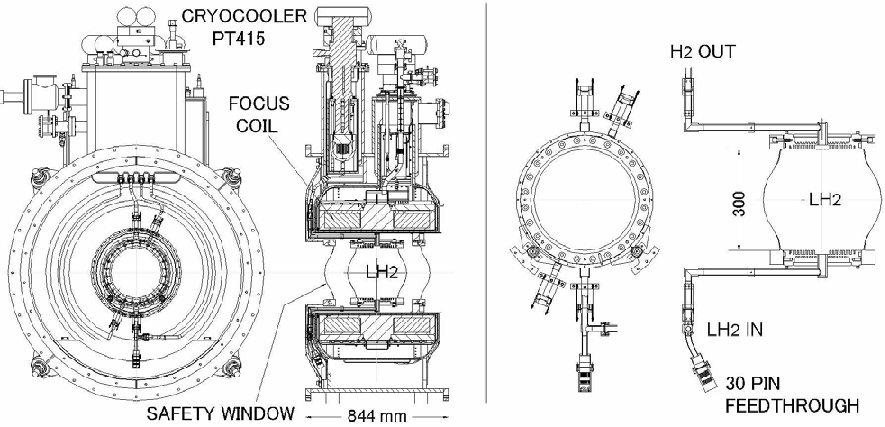
\includegraphics[width=0.75\textwidth]{11-Absorber/Figures/AFC-drwng.pdf}
  \end{center}
  \caption{
    Left panel: Drawing of the absorber/focus-coil (AFC) module showing the principal components. Right panel: detail of the liquid-hydrogen absorber vessel.
  }
  \label{Fig:AbsorberVessel:Diag}
\end{figure}
The absorber vessel was specified to contain 22\,\textit{l} of liquid, so
the body had an inner diameter of 300\,mm and a length between its end
flanges of 230\,mm.  
The length along the central axis between the two domes of the thin aluminium end
windows was 350\,mm.
A detailed description of the construction of the absorber vessel is given in \cite{1748-0221-13-09-T09008}.

The following sections detail the important effects that could contribute to the systematic error of the measured energy loss and scattering in the absorber and thus the cooling effect.

\subsection{Systematic studies}

\subsubsection{Variation of the density of liquid Hydrogen due to varying temperature and pressure}
\label{SubSect:Absorber_temperature}

 The energy lost by a muon travelling through the liquid Hydrogen absorber depends on the path length the
 muon travelled through and on the density of the liquid Hydrogen. The density of liquid Hydrogen changes
 at different temperatures and pressures. To know how much energy the muon lost, we need to accurately know
 the temperature and pressure to determine the density. 
 
 The temperature was recorded by eight LakeShore Cernox 1050 SD sensors. Four of the sensors
 were used solely as temperature sensors, while the other four were used as both temperature and level
 sensors. The level sensors were used when the absorber vessel was being filled to know how much liquid
 Hydrogen was in the vessel and during the experiment to ensure the liquid Hydrogen reached the top of the
 vessel. 

 They were arranged in pairs
 %(Fig.\ref{Fig:AbsorberVessel:BdyPhoto})
 with two mechanically clamped at the
 top of the vessel, two at a rotation of ${45}^{\circ}$, a further two at a further rotation of
 ${90}^{\circ}$ and a final two at a further rotation of ${45}^{\circ}$ to be at the bottom of the vessel.
 The temperature sensors were labelled TSA, TSB, TSD and TSE from top to bottom, while the level sensors
 were labelled LSA, LSB, LSD and LSE from top to bottom.

Cooldown and liquefaction were completed slowly over eight days until the 25 September 2017 at a pressure of 1.15 Bar after which the vessel's pressure was lowered to 1.085 Bar and stabilised during the early hours of the 26 September 2017 \cite{1748-0221-13-09-T09008}. The vessel then remained in this steady-state equilibrium until the 16 October 2017 when the venting process began. During this process the coldhead was switched off and the heaters were switched on, delivering a nominal power of 50 Watt to the absorber vessel. This resulted in an increase in pressure and temperature until it stabilised at the boiling temperature. At this temperature the liquid Hydrogen turned to gas and began emptying from the vessel. A rapid increase in temperature followed once all the liquid Hydrogen had boiled off.

  The sensors have a typical accuracy of $\mathrm{\pm}$ 9mK and a long-term stability of
 $\mathrm{\pm}$ 12mK at 20K. The magnetic field dependent
 temperature error at 2.5T is 0.04\% $\Delta$T/T, equivalent to $\mathrm{\pm}$ 8mK at 20K
 \cite{CernoxRTDs} \cite{TemperatureMeasurement}. These are the quoted uncertainties given by the manufacturer
 of the sensors. The importance of magnetic fields on temperature measurements is that they cause
 reversible calibration shifts. When the magnetic field is removed, the sensors return to their original
 calibration.

 The Cernox 1050 SD sensors only recorded data to a resolution of 0.1 Kelvin for data storage considerations with any following decimal places cut-off and discarded. To be able to compare the temperature and pressure readings at a moment in time and to make the vast amount of data more manageable, a weighted mean was applied to the data \cite{NOTE524}. To reduce the uncertainty in the liquid Hydrogen density a calibration procedure was devised using the boiling point
 (Eq.~\ref{EquationCalibration}). The corrected temperature reading is found by applying a cut-off correction ($c_\textrm{cut-off} = 0.05$), a magnetic field correction based on the focus coil current and mode, and then a boiling point scaling factor. The focus coil correction factors (Table \ref{tab:magnet}) correspond to the slopes when current is plotted against temperature as the magnets are ramped up and down. The temperature coefficient in Eq.~\ref{EquationCalibration} is found by dividing the boiling
temperature reading for that sensor by the boiling temperature of Parahydrogen at that pressure. In Eq.~\ref{EquationCalibration} $I$ is the focus coil current. 
 
\begin{equation}
T_\textrm{corrected}=\frac{T_\textrm{reading}+c_\textrm{cut-off}-c_\textrm{magnet}I}{c_\textrm{Temperature}}
\label{EquationCalibration}
\end{equation}

\begin{table}
\small
  \caption{
    The focus coil current correction coefficients calculated by plotting the temperature against current as the magnets are ramped up and down for each mode, straight and flip. The accuracy of the coefficients is limited by 0.1K resolution
  }
  \label{tab:magnet}
  \begin{center}
    \begin{tabular}{|c c c c c c c c c|}
    \hline

Mode      & LSA & LSB & LSD & LSE & TSA & TSB & TSD & TSE     \rule{0pt}{14pt} \\
\hline
Solenoid & 3.9424E-4 & 4.6810E-4 & 1.2207E-3 & 5.7725E-5 & 7.1284E-5 & 2.8417E-4 & 4.2315E-4 & 3.7478E-4
\\
Flip & 5.5024E-4 & -7.0037E-4 & 9.0778E-4 & 1.8262E-4 & -4.2225E-4 & -6.9633E-4 & -2.0447E-4 & 6.2125E-4
\\

    \hline
    \end{tabular}
  \end{center}
\end{table} 
 
 \begin{table}
\scriptsize
  \caption{
    Temperature coefficient scaling factor for each sensor calculated by dividing the temperature reading (adjusted for cut-off coefficient and magnetic field) by the vaporisation temperature at that pressure
  }
  \label{tab:temperature}
  \begin{center}
    \begin{tabular}{|c c c c c c c c c|}
    \hline

Mode      & LSA & LSB & LSD & LSE & TSA & TSB & TSD & TSE     \rule{0pt}{10pt} \\
\hline
T/T${}_\textrm{Boiling}$ &  1.010581837 & 0.989245608 & 1.003371485 & 1.008424313 & 1.027755673 & 1.003697746 & 0.9784283 & 1.015526132\\

    \hline
    \end{tabular}
  \end{center}
\end{table} 

  \begin{figure}[htb!]
  \begin{center}
    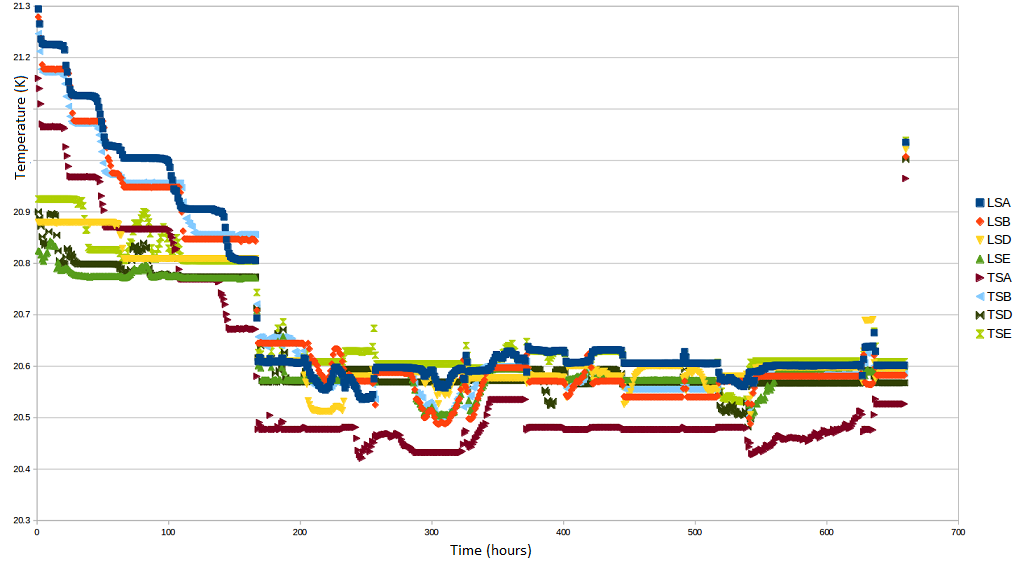
\includegraphics[width=1\textwidth]{TempCalibrated.png}
  \end{center}
  \caption{
    After applying all the correction factors the sensors agree to within 0.2K of each other during the steady state period. During the steady state period the boiling point temperature is 20.511K. Time is given as the number of hours since the 19 September 2017.
  }
  \label{Fig:TempCalibrated}
\end{figure}
 
 The Boiling temperature at 1.085 Bar is 20.511K, with our corrected sensor readings slightly higher (Fig. \ref{Fig:TempCalibrated}). There are however a number of uncertainties. Our readings are recorded to 0.1 K. The sensors add another 29mK (9mK accuracy + 12mK stability + 8mK magnetic field), although the magnetic field error is likely greater. The temperature scaling and magnet current correction factors also have an associated error as they are based on the 0.1K resolution. For example, a calibrated sensor at boiling temperature and 1.505 Bar should read 21.692K but can only read 21.65K (21.6K cut-off plus 0.05 cut-off correction) i.e. it is off by 0.042K. The pressure sensors have an uncertainty of $\mathrm{\pm}$ 5mBar which equates to $\mathrm{\pm}$ 0.016K during steady state. The pressure uncertainty ($\mathrm{\pm}$ 5mBar) adds another uncertainty to the temperature calibration constants of $\mathrm{\pm}$ 0.014K. Collectively, all these uncertainties add up to 0.2K.
 
 Knowing that in our steady state condition the liquid Hydrogen was close to the boiling temperature of liquid Parahydrogen  \cite{NOTE524} at 20.5K $\mathrm{\pm}$ 0.2K and 1.085 Bar allows us to determine the uncertainty in the density as 70.54kg/m${}^{3}$ $\mathrm{\pm}$ 0.24kg/m${}^{3}$
 

\subsubsection{Contraction of the absorber vessel due to cooling}
\label{SubSect:Absorber_Contraction}

The Aluminium absorber vessel was cooled from room temperature to the operating temperature of the
experiment ($\mathrm{\approx}$20.3K), which resulted in the vessel contracting. The linear contraction of
Al-6061 as it is cooled from 293K is given by the equation

\begin{equation}
  \alpha =-4.1277\times {10}^{-3}T-3.0389\times {10}^{-6}T^2+8.7696\times {10}^{-8}T^3-9.9821\times {10}^{-11}T^4
\end{equation}
where T is the operating temperature \cite{Hardin}. The equation is a line of best fit of data collated by NIST
(National Institute of Standards and Technology) and has an associated curve fit error of 4\%.

At the MICE operating temperature, this corresponds to a linear contraction of the vessel along each plane of 0.415\%
(293K $\mathrm{\to}$ 20.3K), resulting in a warm bore length (350mm) contraction of 1.4525mm
$\mathrm{\pm}$ 4\%. The vessel was held suspended in place, meaning the vessel was free to contract along
each plane without restriction, ensuring there were no forces created to distort the shape of the vessel.


\subsubsection{Deflection of absorber vessel windows due to internal pressure}
\label{SubSect:Absorber_pressure}

To minimise energy loss and Coulomb scattering by the absorber vessel, the windows were kept as thin as
possible. They must however not rupture when handling any internal pressure they are subjected to. For
safety considerations \cite{1748-0221-13-09-T09008} \cite{Ishimoto} it is necessary for the liquid hydrogen
circuit to be pressurised above atmospheric pressure to prevent air ingress. The vessel must also be
capable of handling up to 1.5 Bar, the relief valve set pressure.

These pressures resulted in a deflection of the absorber windows and were modelled by Green and Yang using
ANSYS \cite{NOTE155}. The uncertainty in the model's window deflection was 20\%. It showed a linear
expansion of the window deflection with pressure up to 2 Bar when the windows begin to yield. 

 The pressure sensors are accurate to $\mathrm{\pm}$ 5mBar (0.25\% of 2 BarA Full Scale). At 1085
 $\mathrm{\pm}$ 5 mBar, the typical MICE operating pressure, this corresponds to a deflection of 0.5374mm
 $\mathrm{\pm}$ 0.1076mm (model uncertainty) $\mathrm{\pm}$ 0.0022mm (sensor uncertainty) at the centre of
 the absorber window.


\subsubsection{Variation of the absorber vessel window thicknesses}
\label{SubSect:Absorber_thickness}

The amount of energy loss and cooling experienced by a muon passing through the absorber depends on the amount of
Aluminium and liquid Hydrogen traversed. There are four windows, two absorber wall windows of the vessel and two safety windows.
%(Windows 002, 003, 009 and 012 from Table \ref{tab:summary}) 

At the centre of the absorber, the
total amount of Aluminium the muon beam passes through is 785 $\mathrm{\pm}$ 24 microns, a variance of
3.057\%. However, as the windows are thin, the effects on energy loss are negligible. A 200MeV muon passing
along the central axis of an empty absorber loses 0.345 MeV, which introduces a 0.01 MeV uncertainty on
energy loss.


\subsubsection{Total Systematic Uncertainty on Energy Loss}
\label{SubSect:Absorber_total}

In total there are three main contributions to the systematic uncertainty of the liquid Hydrogen absorber on energy loss. The contraction of the absorber and deflection of the absorber window due to internal pressure (Eq.~\ref{Totaldeflection}) reduces the central warm bore length by 0.4 $\mathrm{\pm}$ 0.3mm.

\begin{equation}
    1.4525\ \left(\pm \ 0.0581\right)-2\left(0.5374\left(\pm 0.1098\right)\right)=0.3777\pm 0.2777=0.4mm\pm 0.3mm
\label{Totaldeflection}    
\end{equation}

The combined absorber window thickness variation at the centre of the absorber is 24 microns. The temperature during the steady state period of the experiment when the pressure remained constant at 1085 $\mathrm{\pm}$ 5 mBar is 20.5 $\mathrm{\pm}$ 0.2K corresponding to a liquid Hydrogen density of 70.54 $\mathrm{\pm}$ 0.24kg/m${}^{3}$.

The energy loss is momentum dependent as each particle will lose a different amount of energy passing through the absorber. Tables \ref{tab:Aluminium} and \ref{tab:Hydrogen} show the energy loss at various momenta and densities of Aluminium and liquid Hydrogen \cite{AtomicAluminium} \cite{AtomicHydrogen} \cite{MuonAluminium} \cite{MuonliquidHydrogen}. 277 MeV and 344 MeV are the minimum ionization momenta of Aluminium and liquid Hydrogen respectively.


\begin{table}[h]
  \caption{
    Energy Loss for Aluminium (Al-6061) at various momenta with a density of 2.699 g/cm${}^{3}$.
  }
  \label{tab:Aluminium}
  \begin{center}
    \begin{tabular}{|c c c c c|}
    \hline

Momentum (MeV) & 100 & 140 & 200 & 277     \rule{0pt}{14pt} \\
\hline
{Mass Stopping Power (MeVg${}^{-1}$cm${}^{2}$)} & 1.798 & 1.688 & 1.630 & 1.615
\\
{Stopping Power (MeVcm${}^{-1}$)} & 4.8528 & 4.556 & 4.3994 & 4.3589
\\

    \hline
    \end{tabular}
  \end{center}
\end{table} 

\begin{table}
  \caption{
    Energy loss for liquid Hydrogen at various densities (0.0703 to 0.0708 g/cm${}^{3}$) and various momenta of muons.
  }
  \label{tab:Hydrogen}
  \begin{center}
    \begin{tabular}{|c c c c c|}
    \hline

Momentum & 100 & 140 & 200 & 344     \rule{0pt}{14pt} \\
\hline
{Mass Stopping Power} & 4.568 & 4.267 & 4.104 & 4.034 \\
{Stopping Power }(at $\rho$=0.0703)\textbf{} & 0.3211 & 0.29997 & 0.2885 & 0.28359\\
{Stopping Power }(at $\rho$=0.07054)\textbf{} & 0.3222 & 0.30099 & 0.2895 & 0.2846 \\
{Stopping Power }(at $\rho$=0.07078)\textbf{} & 0.3233 & 0.3020 & 0.29048 & 0.2855 \\
{Stopping Power }(at $\rho$=0.0708)\textbf{} & 0.3234 & 0.3021 & 0.29056 & 0.2856 \\
    \hline
    \end{tabular}
  \end{center}
\end{table} 


 During the MICE experiment 140, 170, 200 and 240 MeV momenta muon beams were used. The energy loss and its uncertainty were then be calculated. The calculation used a central bore length of 349.6 $\mathrm{\pm}$ 0.3mm, a total window thickness of 0.785 $\mathrm{\pm}$ 0.024mm and a liquid Hydrogen density of 70.54 $\mathrm{\pm}$ 0.24kg/m${}^{3}$ for a particle travelling straight through the centre of the absorber.

 For a 140 MeV muon particle this corresponds to an energy loss of 10.88 $\mathrm{\pm}$ 0.06 ($\mathrm{\pm}$ 0.51\%) MeV, while for a 200 MeV muon particle this corresponds to an energy loss of 10.44 $\mathrm{\pm}$ 0.05 ($\mathrm{\pm}$ 0.51\%) MeV. In terms of Energy loss, the systematic error is 0.51\%. This is for a particle travelling along the central axis of the absorber. An actual muon travelling through the absorber with a magnetic field will take a different path and thus have a different path length of Aluminium and liquid Hydrogen traversed.
 
%%%%%%%%%%%%%%%%%%%%%%%%%%%%%%%%%%%%%%%%%%%%%%%%%%%%%%%%%%%%%%%%%%%55 
% Scott's section 
%\subsection{Systematic effect on the Scattering Analysis}
%\label{SubSect:Absorber_E}

\subsection{Validation of the absorber model in MAUS}
\label{SubSect:Absorber_Validation}

As a test of the absorber model, an analysis has been performed to measure the muon energy loss in the LiH and liquid Hydrogen absorbers and compare it to the energy loss predicted by the MC.  A previous analysis measured this effect using only the TOF detectors~\cite{rhys_thesis} and found good agreement in the mean energy loss, but did not have the precision to measure the shape of the distribution.  In this updated energy loss analysis, the addition of the trackers allows better PID, slightly improved momentum measurements upstream compared to the TOF0-TOF1 measurement, and significantly improved momentum measurements downstream compared to the TOF1-TOF2 estimate.

Muons are selected using the particle ID described in Section~\ref{Sect:PID}.  The muons' upstream momentum (before the absorber) is measured using an average of the momentum measured by the tracker (at the plane nearest to the absorber) and the momentum calculated using the TOF0 to TOF1 flight time.  This average is weighted by the expected resolution of the two measurements. (The resolutions are roughly the same for low-momentum muons, but the TOF measurement of momentum is less accurate for higher-momentum muons.)  The muons' downstream momentum is measured solely using the dowstream tracker.

The momentum change is measured for each beam momentum both with and without an absorber present.  The LiH `empty' measurement is done with no absorber present, while the liquid Hydrogen `empty' measurement is done with the hydrogen vessel in place, but not filled.  The measurement with no absorber is used to find the resolution of the detector, and the measurement with a full absorber should then be a convolution of the true loss in the absorber and this resolution.

In order to extract the true momentum loss in the absorber, the `empty absorber' result is modeled by a gaussian distribution.  The `full absorber' measurement is then fit to a convolution of a the true momentum loss (a landau distribution with free parameters) and the resolution of the detector (a gaussian distibution with parameters fixed by the `empty absorber' fit).

\begin{figure}
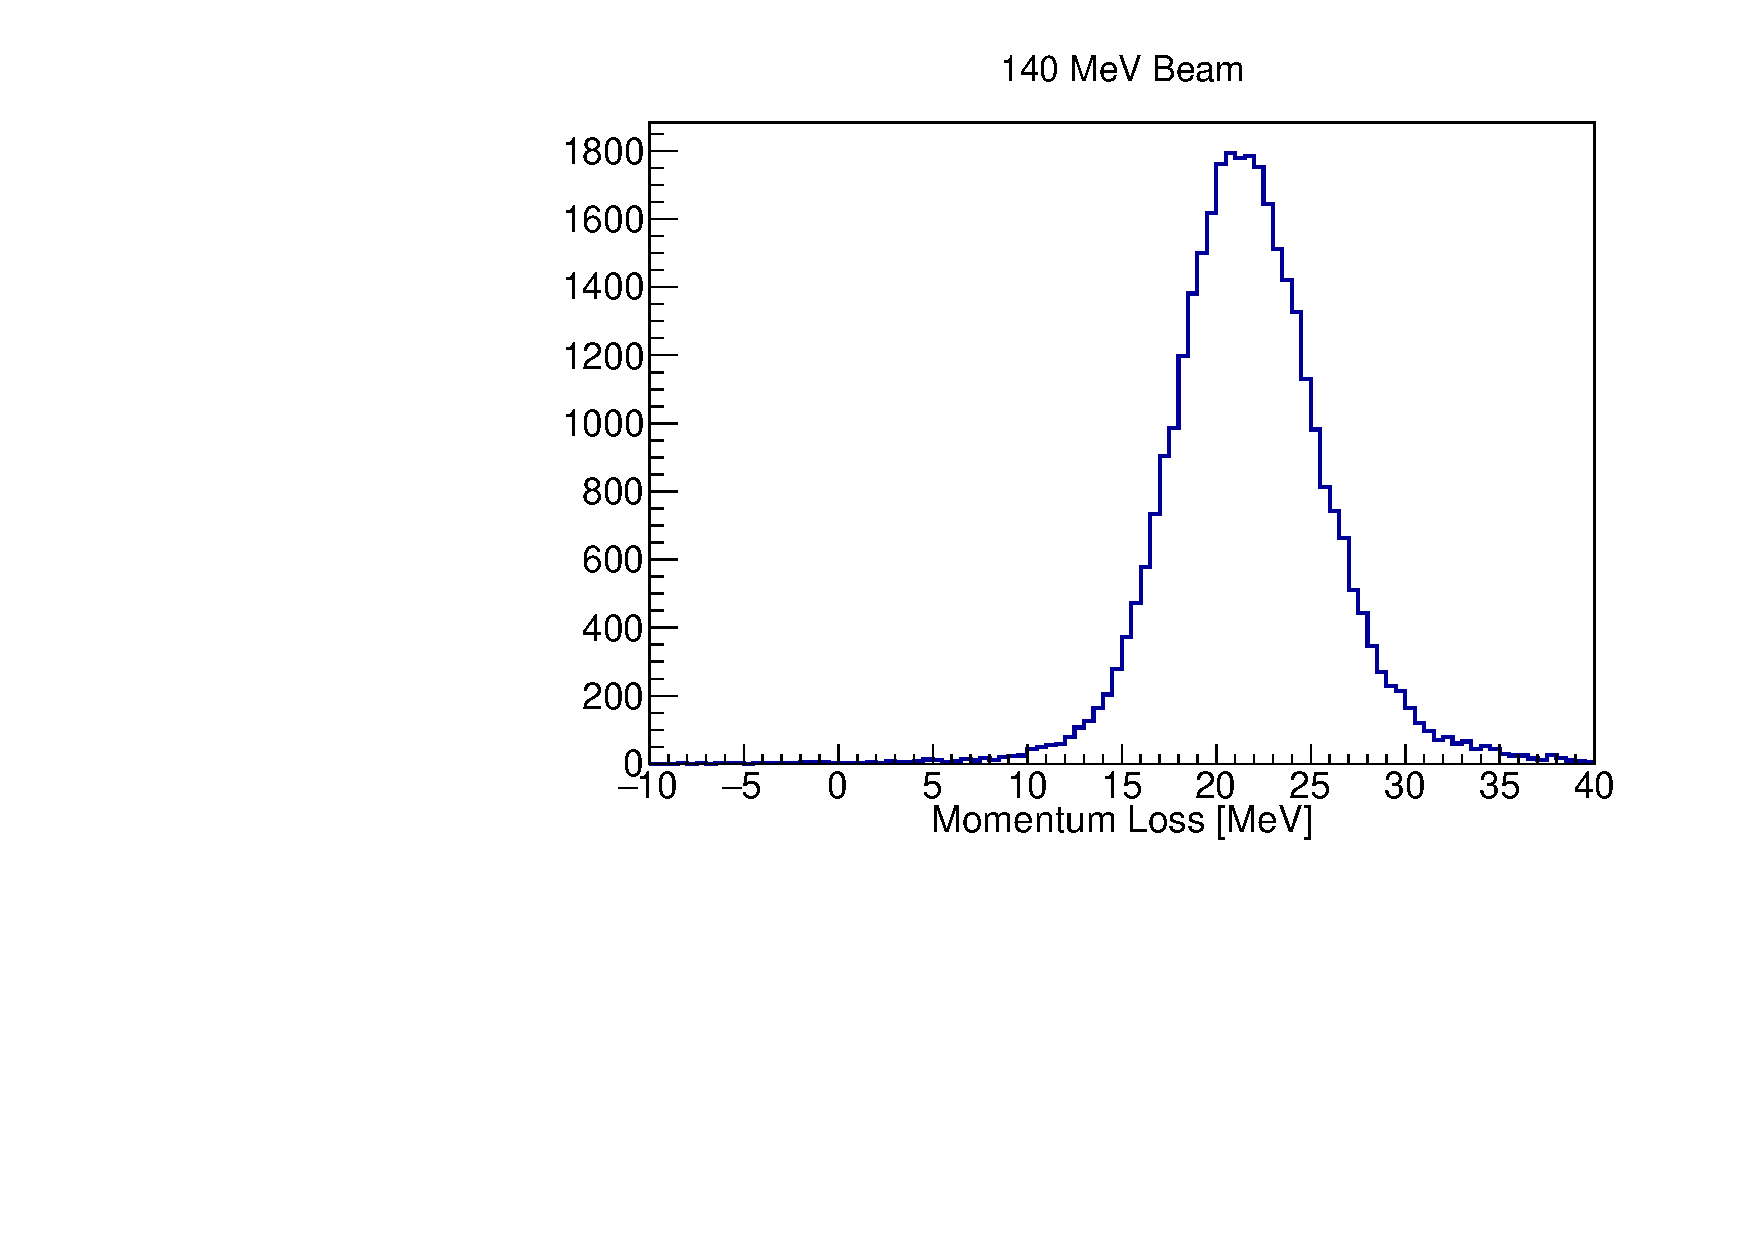
\includegraphics[width=0.45\textwidth]{11-Absorber/Figures/raw_140.pdf}\hfil
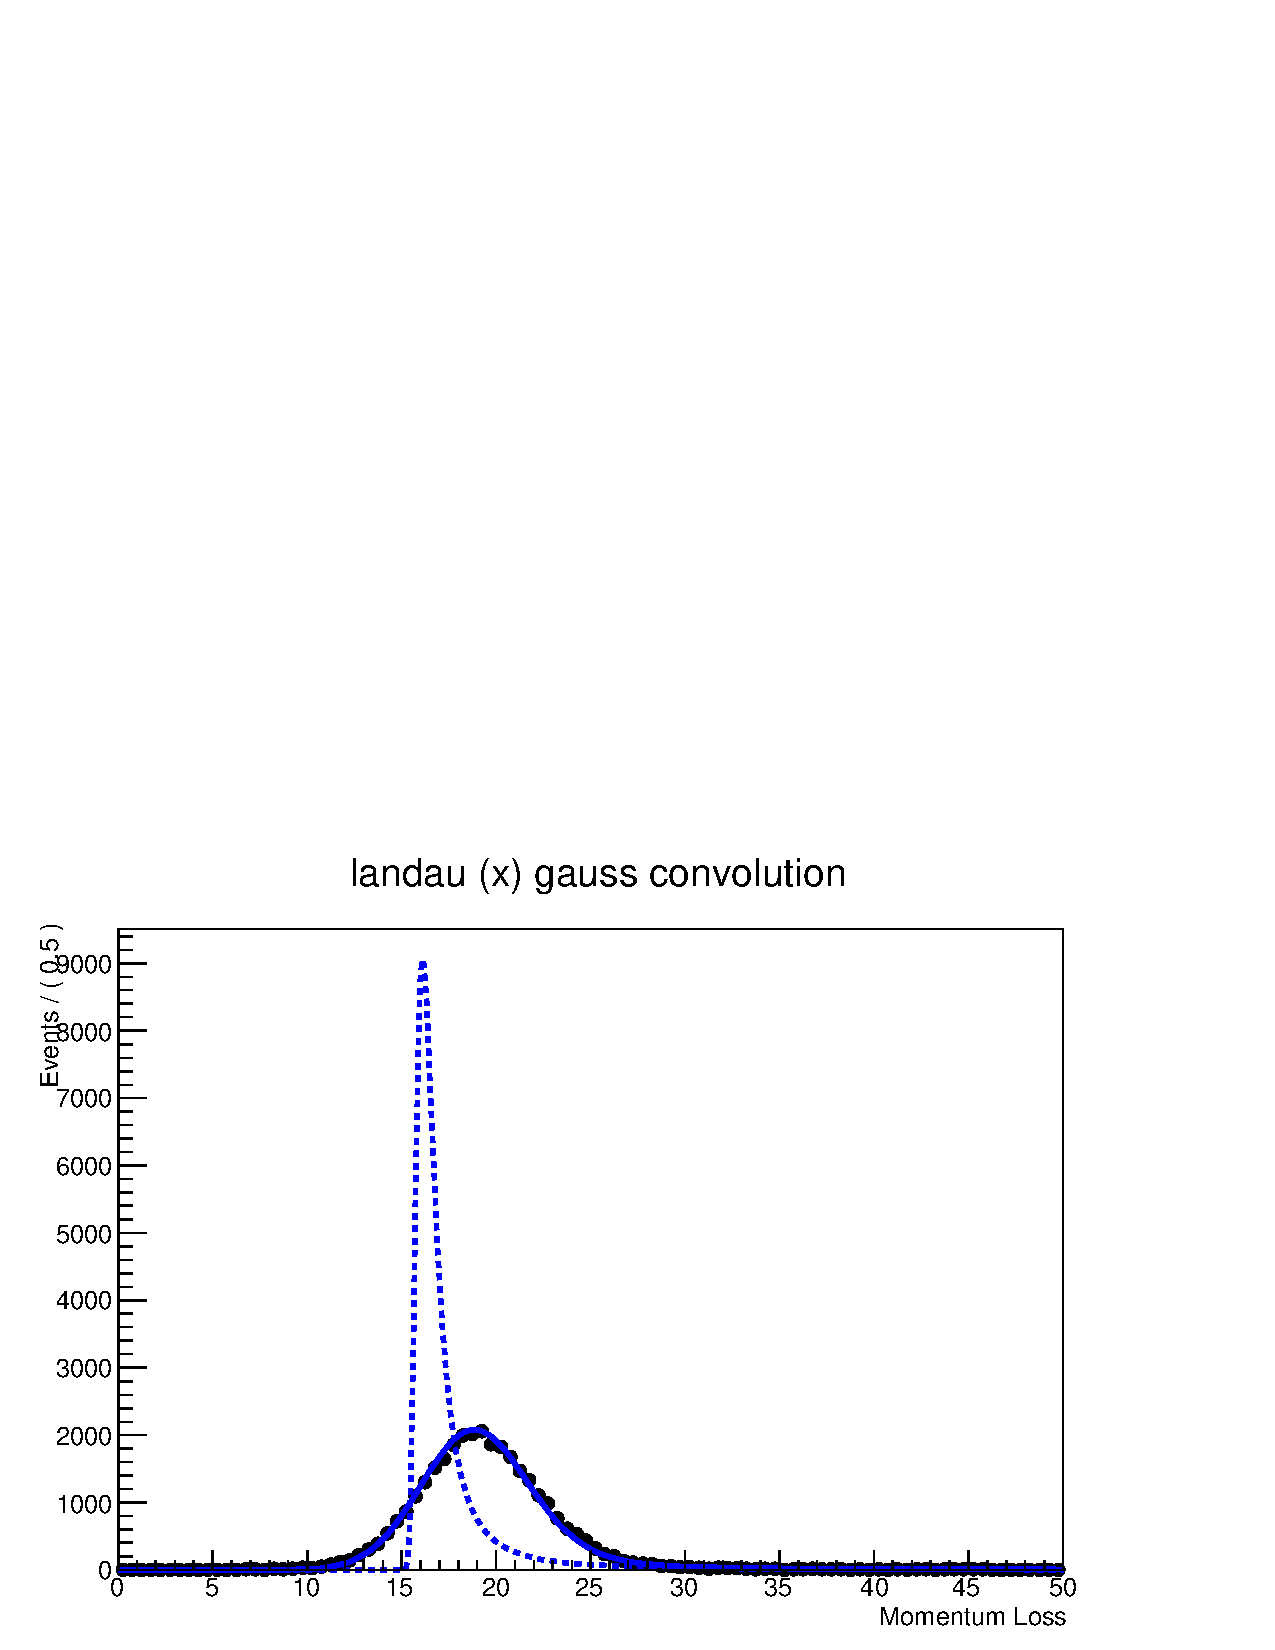
\includegraphics[width=0.45\textwidth]{11-Absorber/Figures/deconv_140.pdf}
\vspace{-5cm}

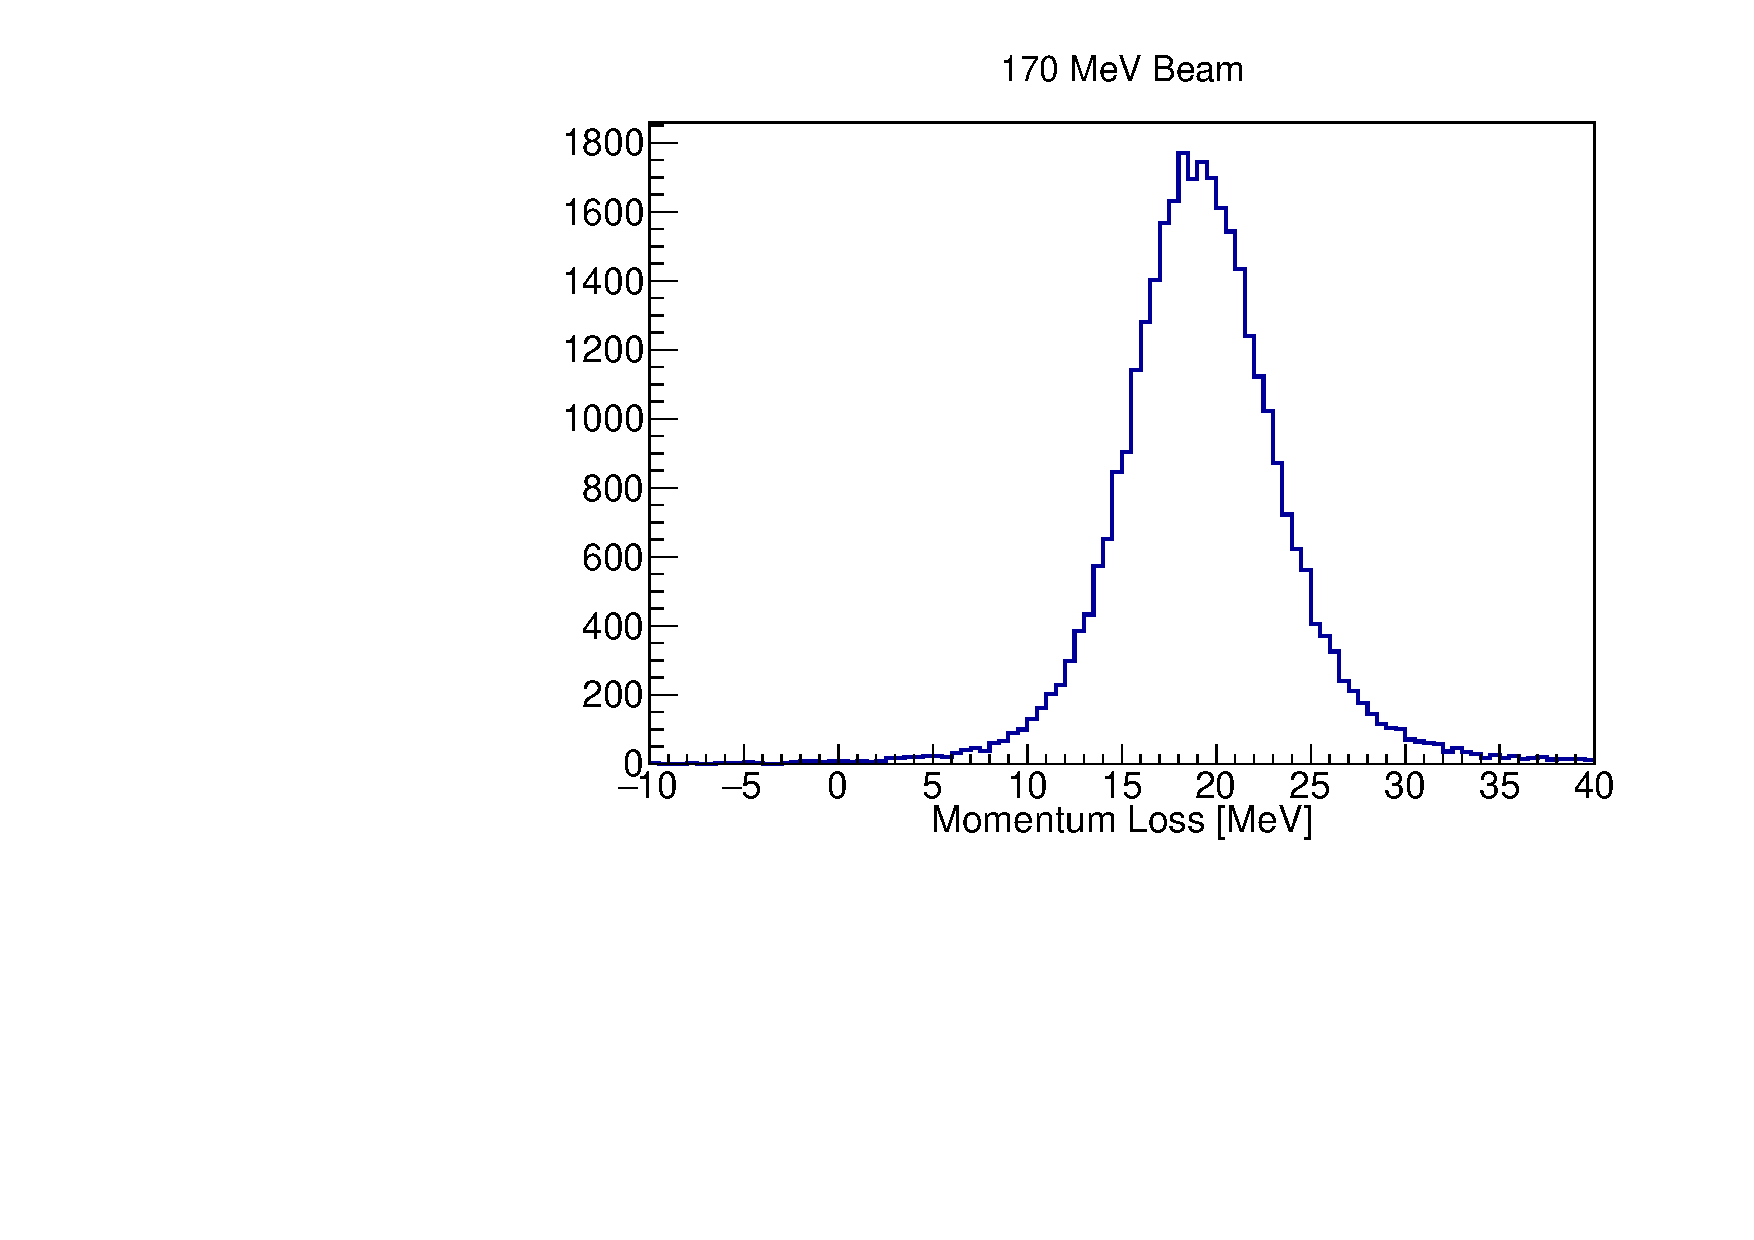
\includegraphics[width=0.45\textwidth]{11-Absorber/Figures/raw_170.pdf}\hfil
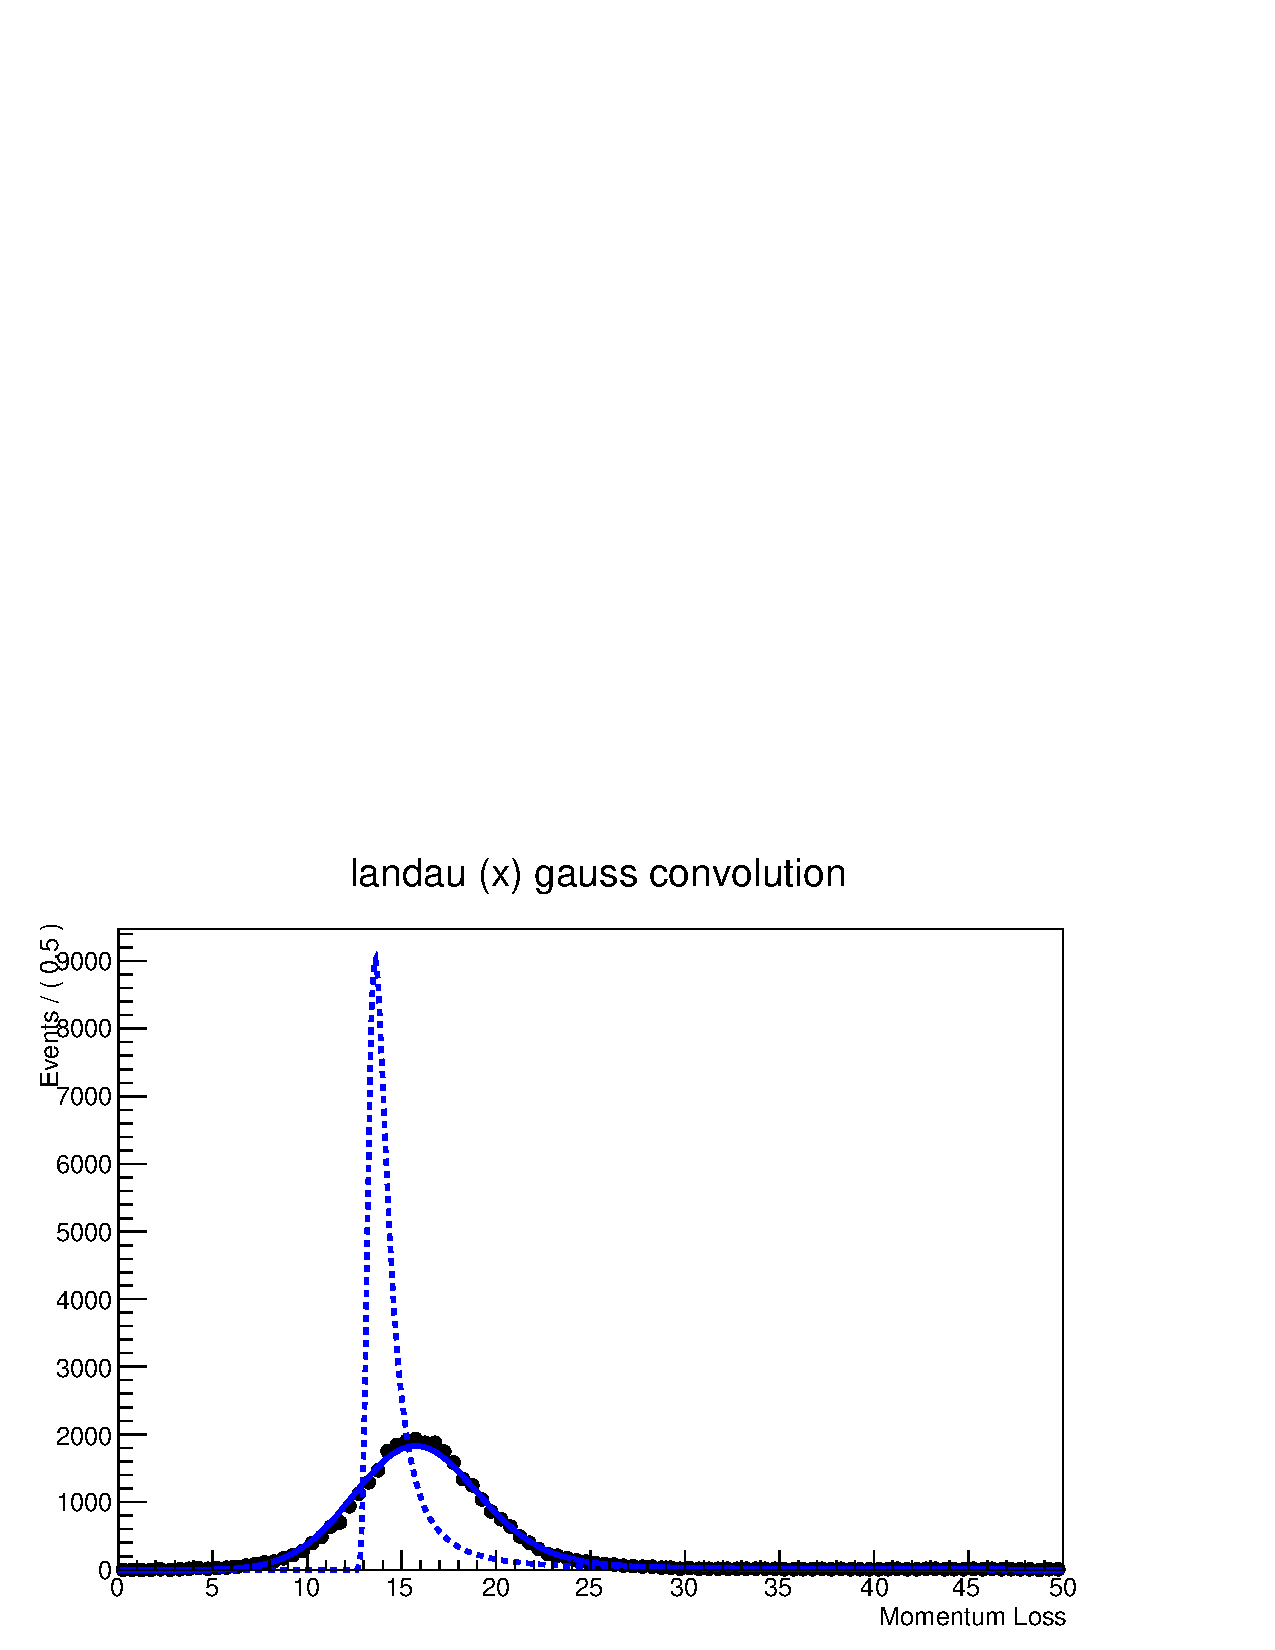
\includegraphics[width=0.45\textwidth]{11-Absorber/Figures/deconv_170.pdf}
\vspace{-5cm}

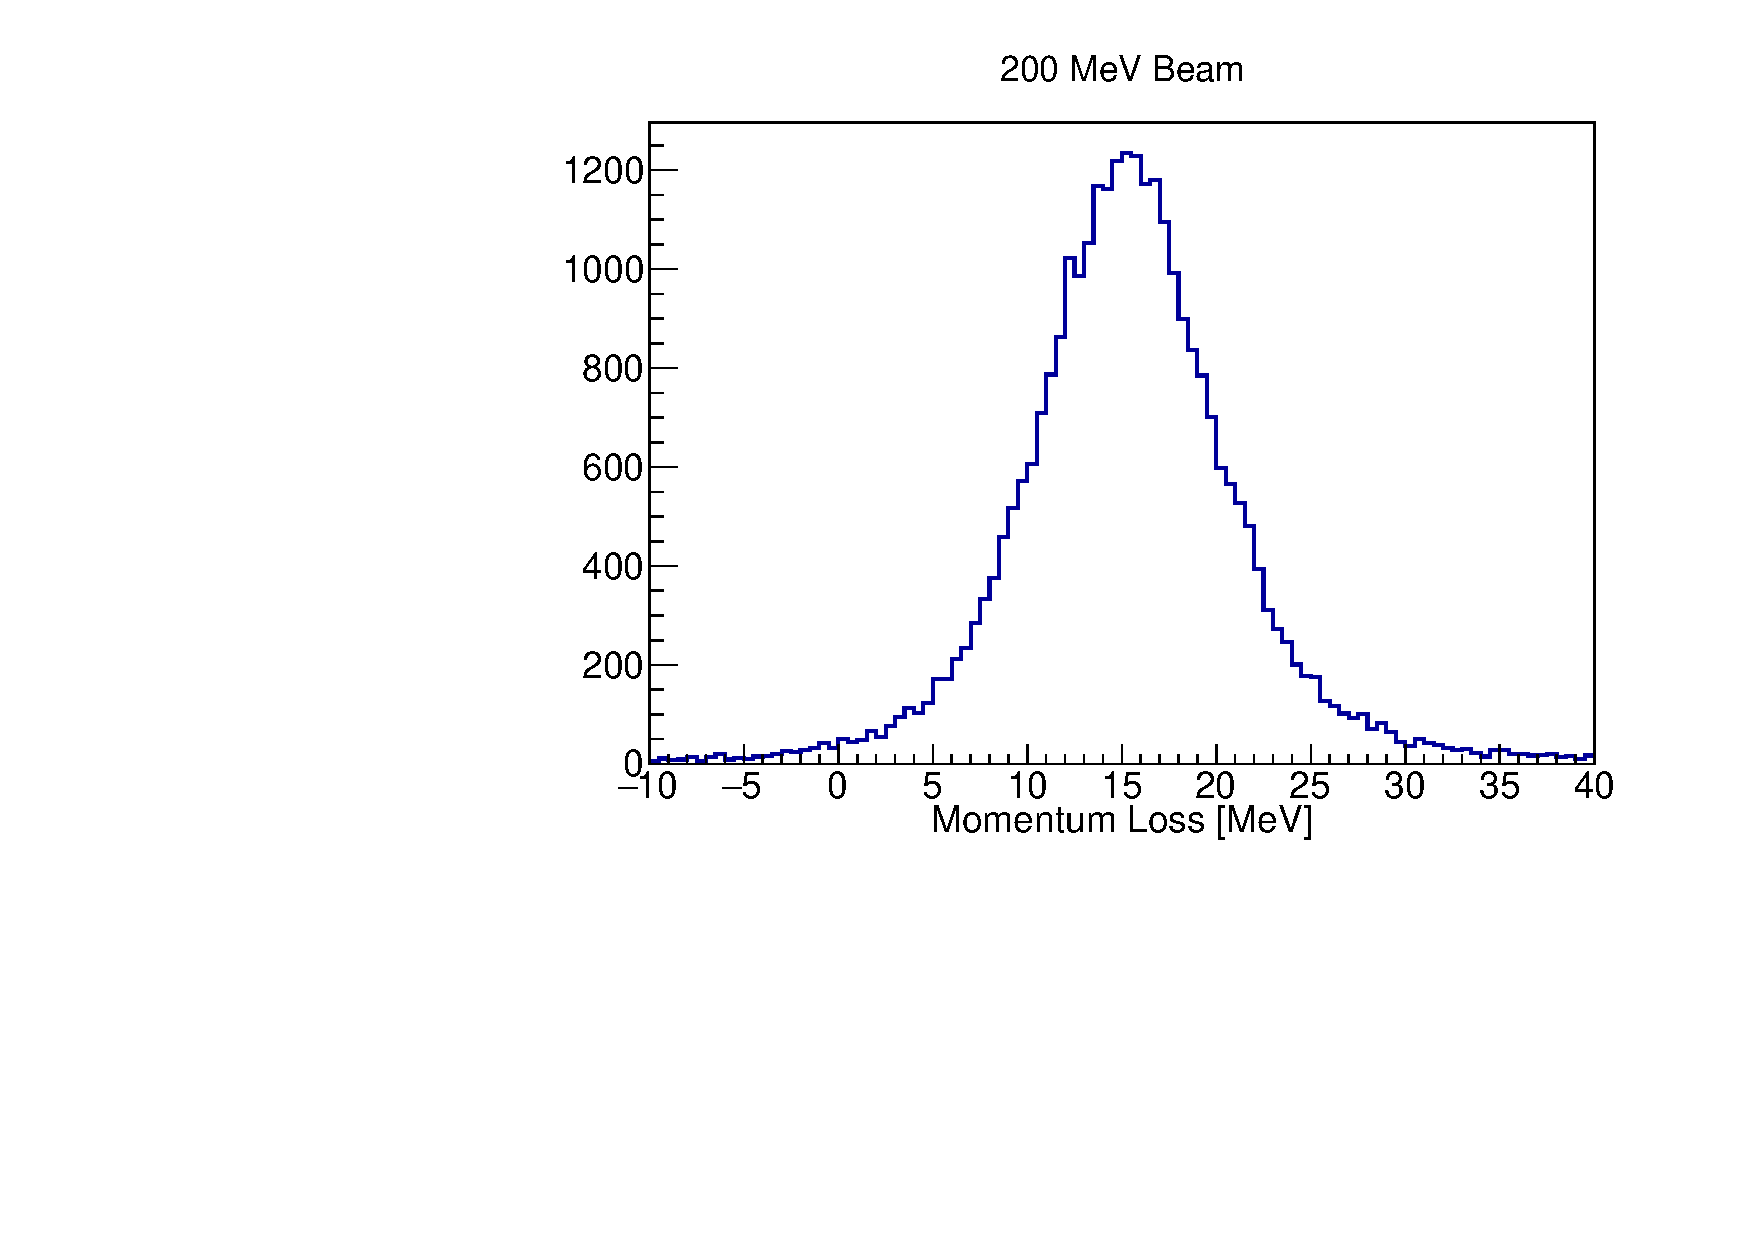
\includegraphics[width=0.45\textwidth]{11-Absorber/Figures/raw_200.pdf}\hfil
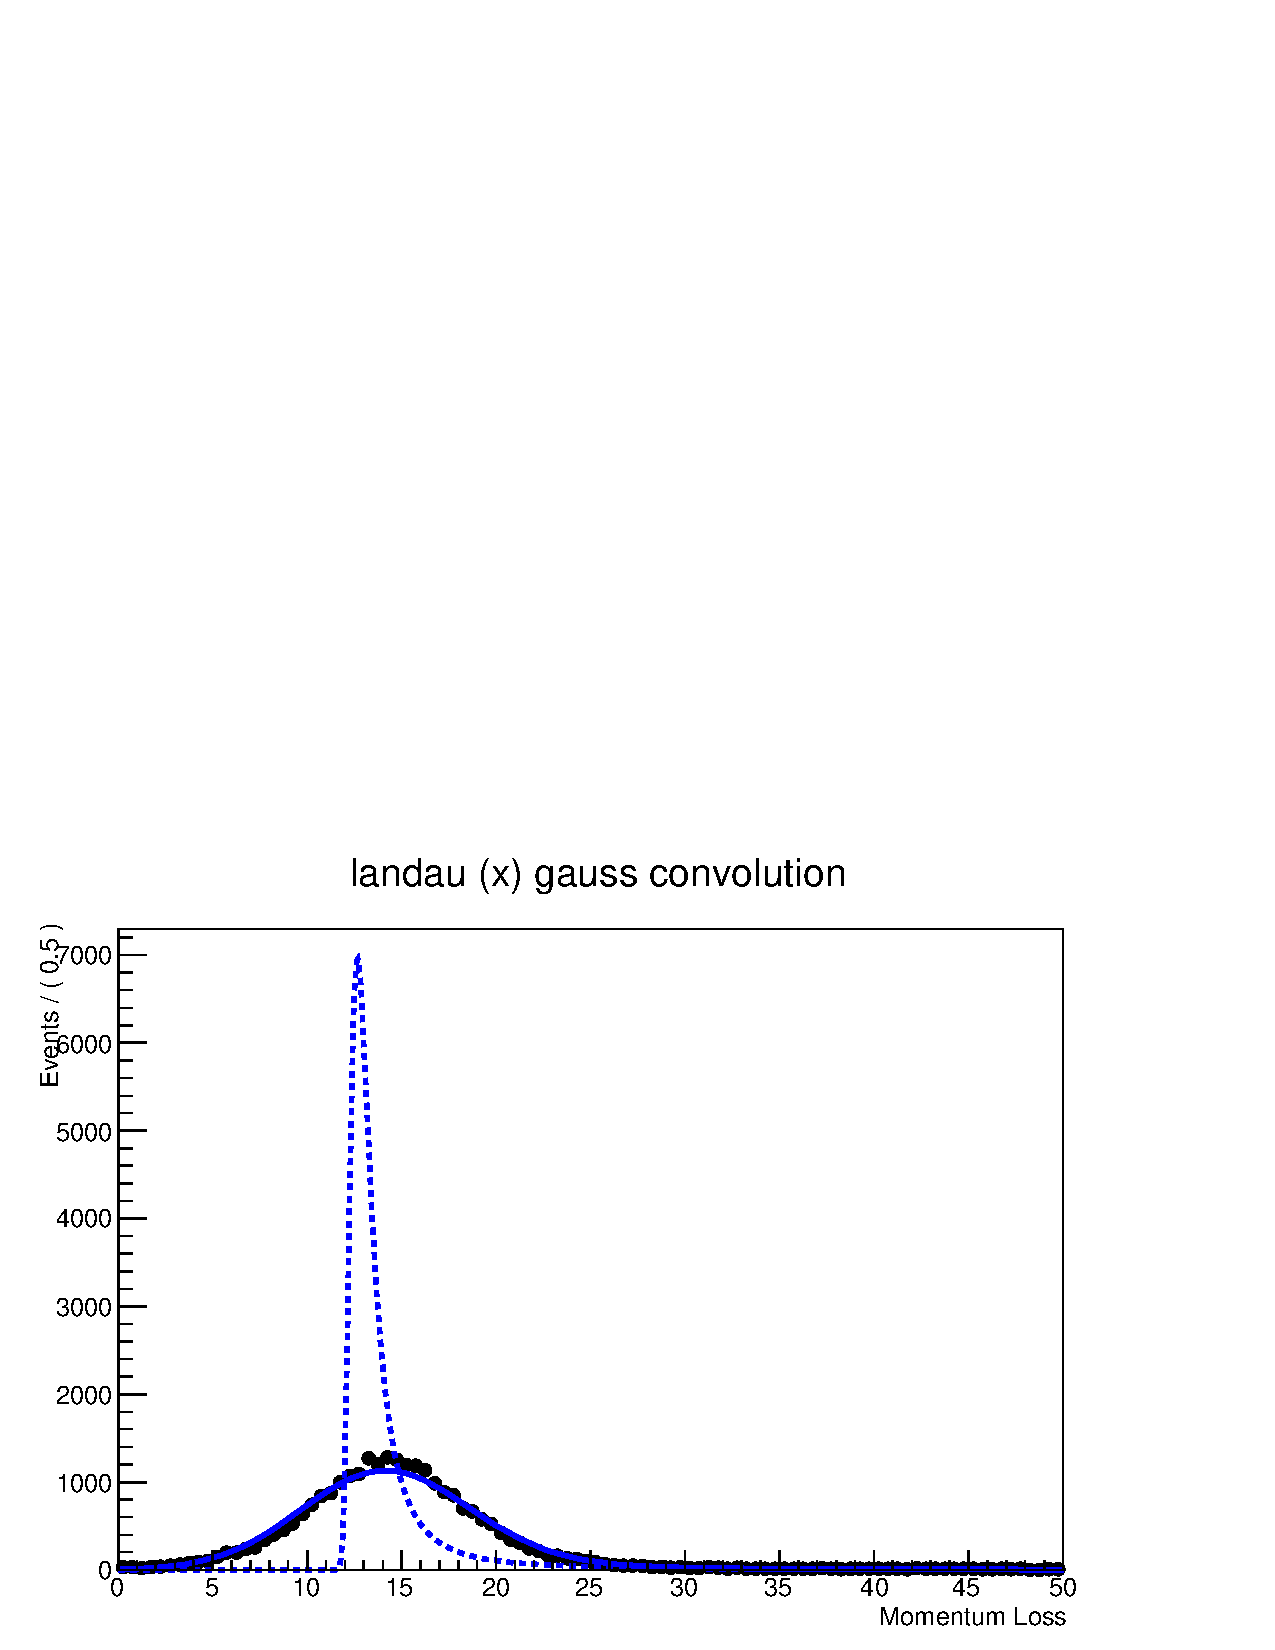
\includegraphics[width=0.45\textwidth]{11-Absorber/Figures/deconv_200.pdf}
\vspace{-5cm}

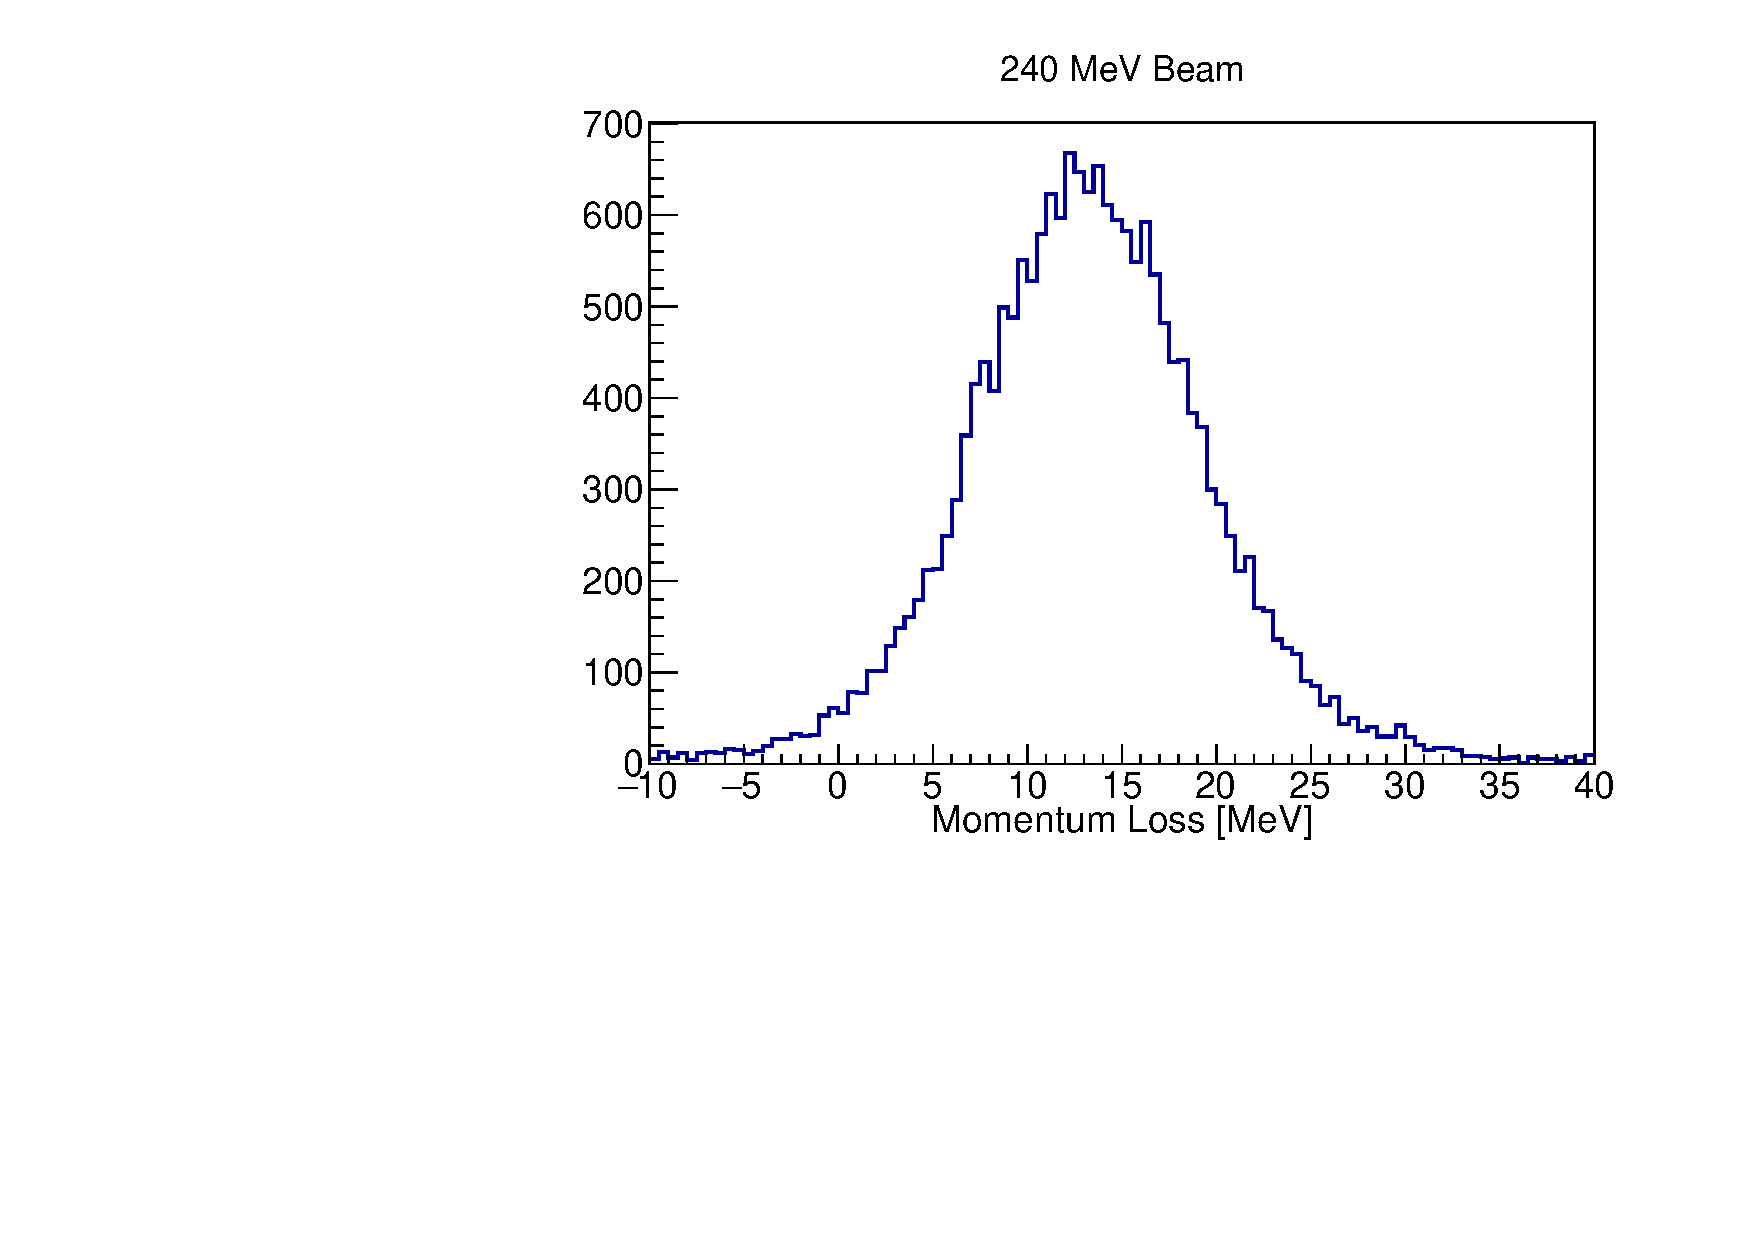
\includegraphics[width=0.45\textwidth]{11-Absorber/Figures/raw_240.pdf}\hfil
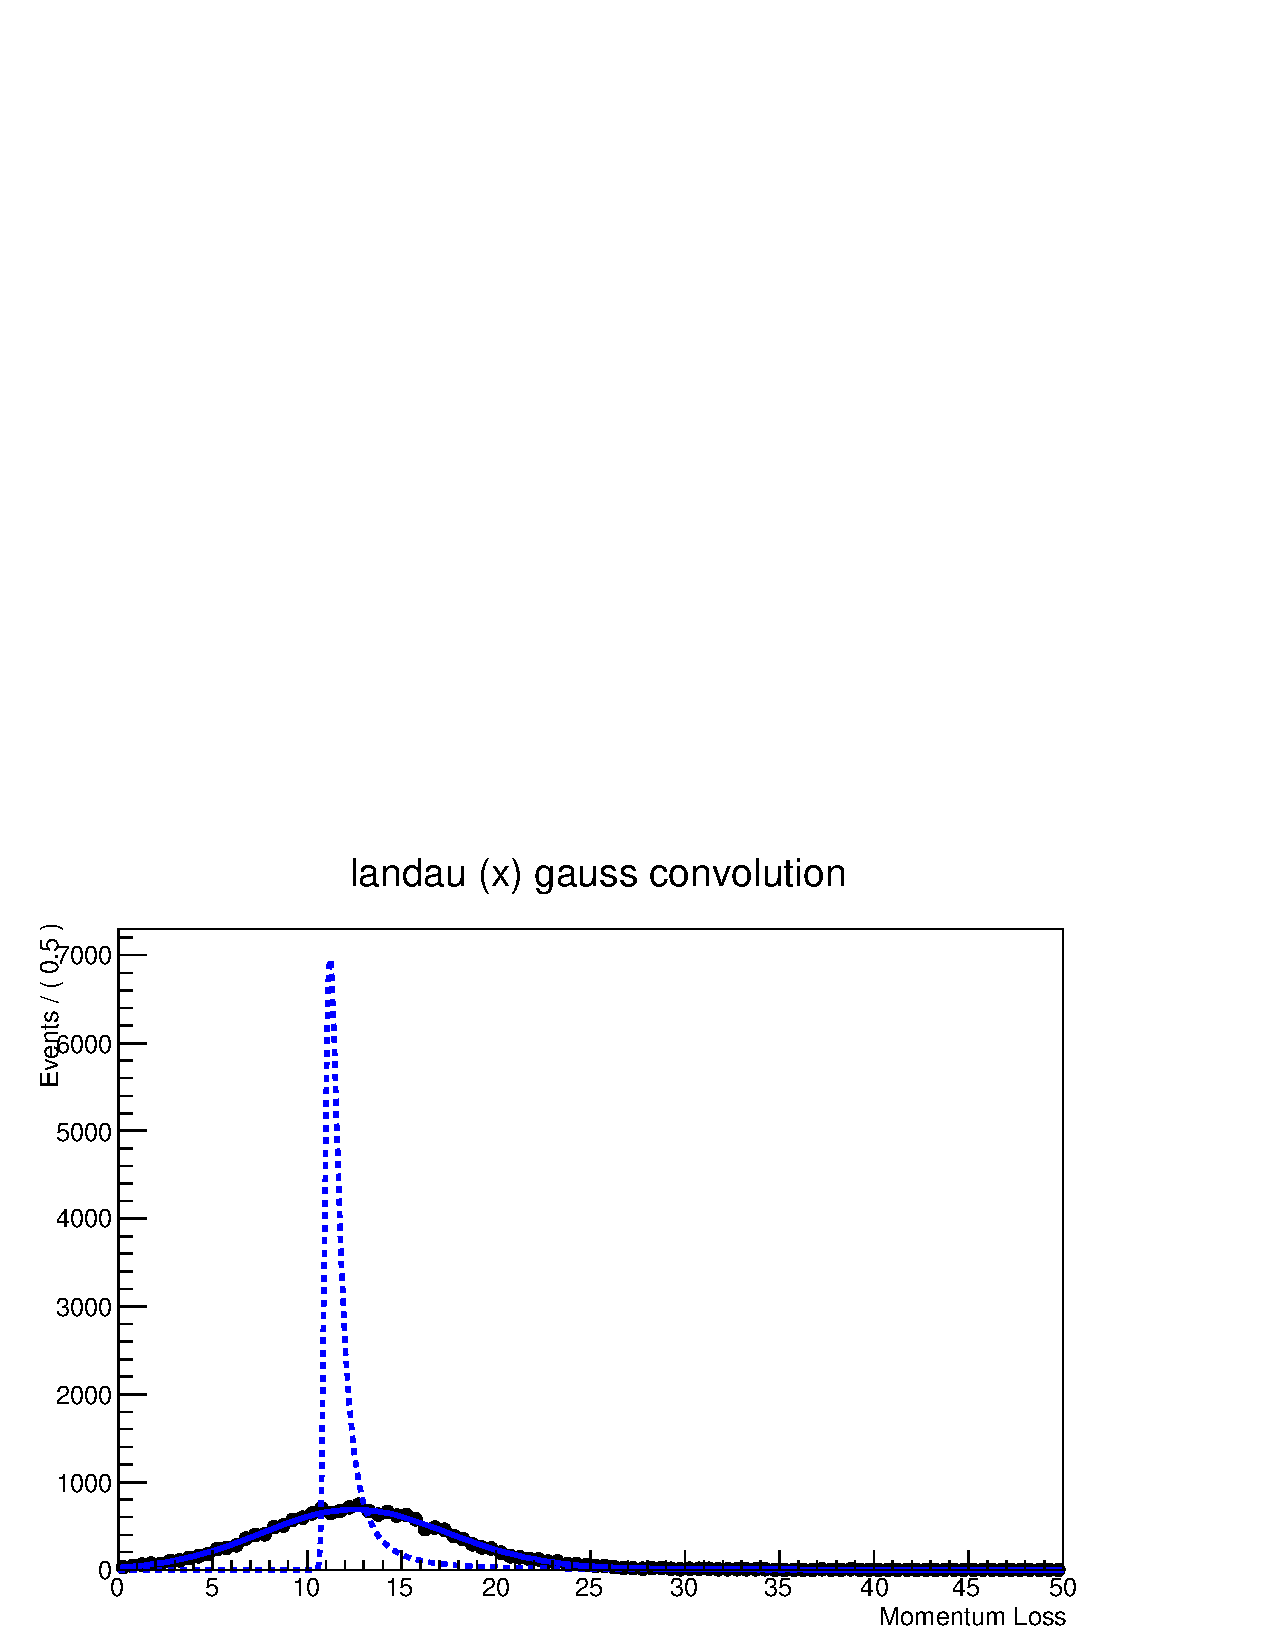
\includegraphics[width=0.45\textwidth]{11-Absorber/Figures/deconv_240.pdf}
\caption{\label{fig:eloss_data} The measured momentum loss (left) and deconvolved distributions (right) in the MICE Lithium Hydride absorber.  Four different momentum settings are shown: 140 MeV(a), 170 MeV(b), 200 MeV(c), and 240 MeV(d).  The `deconvolved' plots show the data (black points), the fitted convolved landau and gaussian (solid blue line) and the landau by itself (dotted blue line).}
\end{figure}

The measurement of momentum loss is taken at four different beam momenta.  It agrees well with the Monte Carlo (in which the energy loss is modeled by GEANT) and with the predictions of the Bethe-Bloch formula, as shown in Figure~\ref{fig:eloss_bb}.

{\color{red}
\begin{itemize}
\item add LH2 plots
\item systematics
\item more words about comparing with MC and Bethe-Bloch
\end{itemize}
}

\begin{figure}
\hfil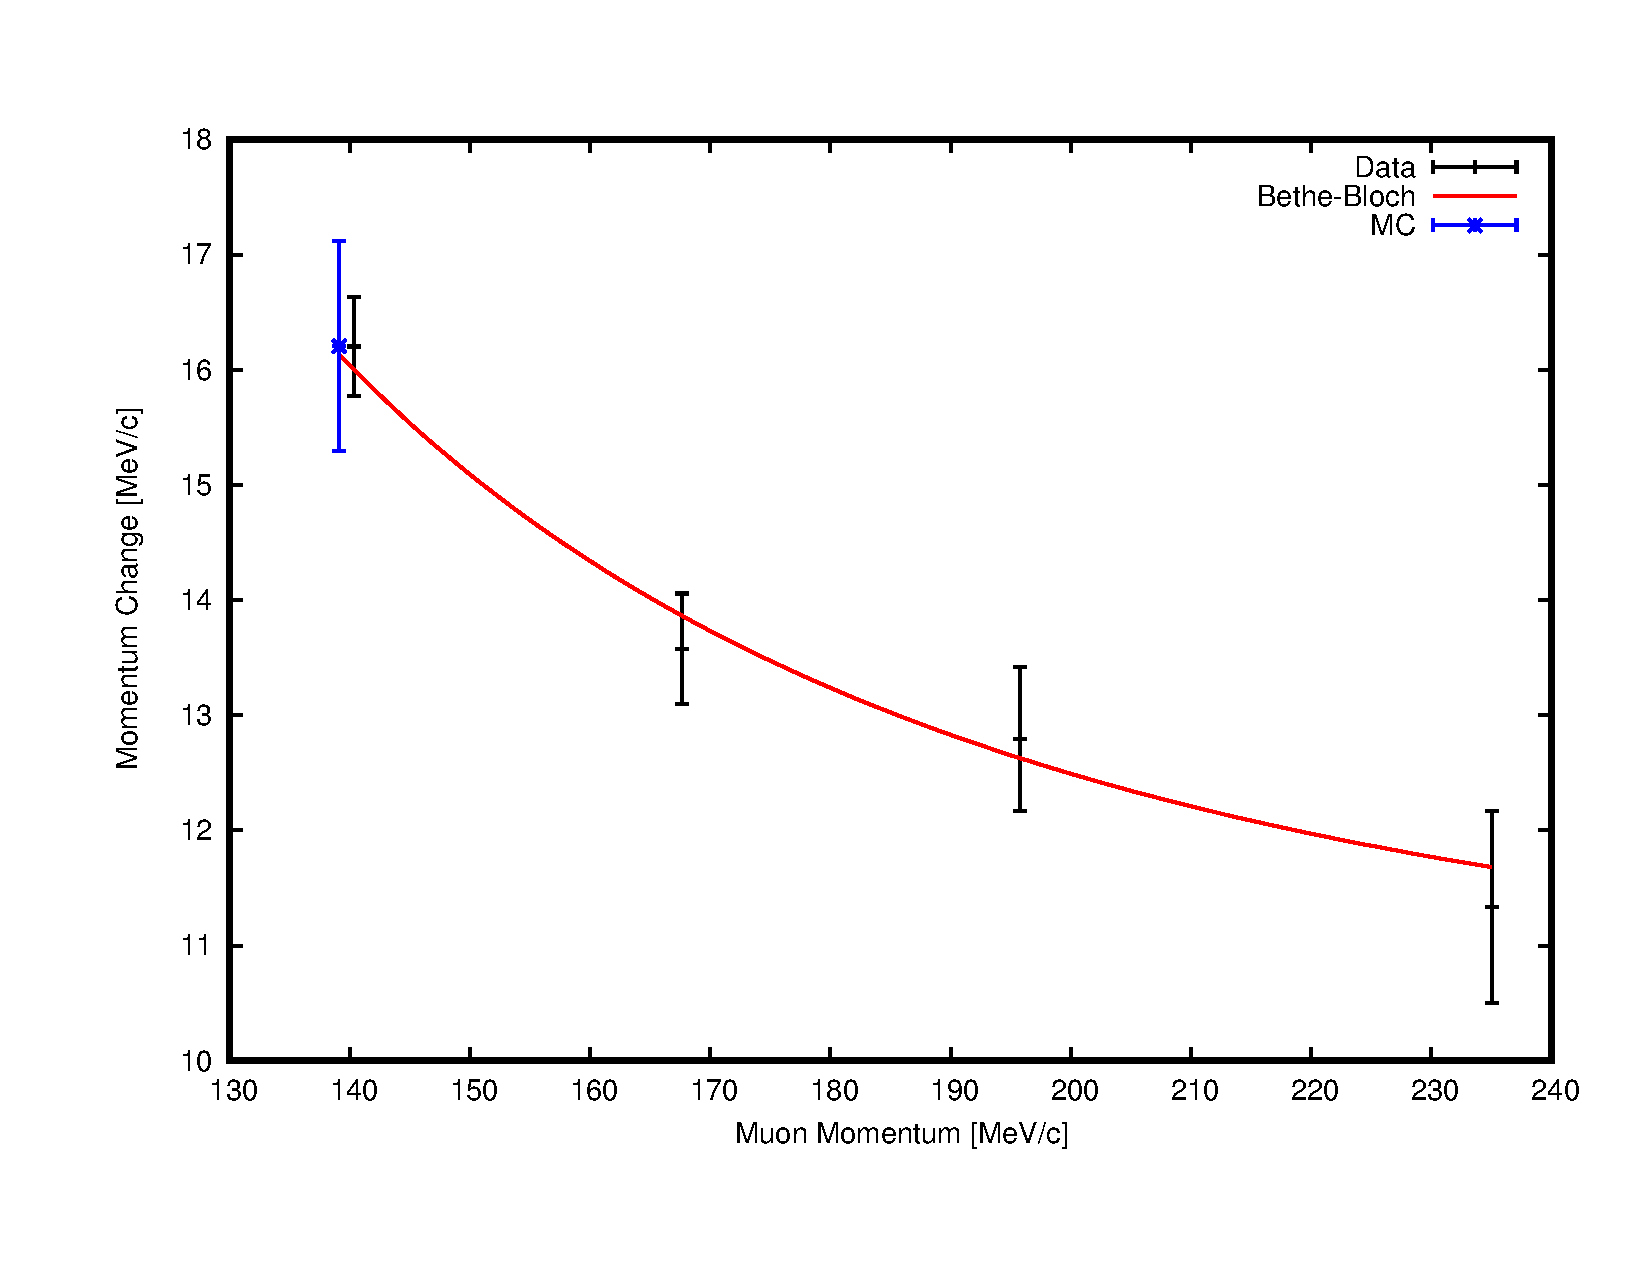
\includegraphics[width=0.45\textwidth]{11-Absorber/Figures/bb_compare.pdf}\hfil

\caption{\label{fig:eloss_bb} Comparison of measured momentum loss in data and in MC in Lithium Hydride.  MPV of momentum loss is shown at each point with the predition from the Bethe-Bloch formula shown as a solid line.}
\end{figure}


%% Effect of error in geometry
%%   Test firing particles with modified geometry.
%%   Modified geometry in Scott's analysis.
